%%%%%%%%%%%%%%%%%%%%%%%%%%%%%%%%%%%%%%%%%%%%%%%%%%%
% Poster for Epigenetics course, Curie Paris 2013 %
% Author: Ricky Lim                               %
% Supervisor: Guillaume Filion                    %
%%%%%%%%%%%%%%%%%%%%%%%%%%%%%%%%%%%%%%%%%%%%%%%%%%%


% preamble
\documentclass[serif,mathserif,final]{beamer}
\mode<presentation>{\usetheme{Lankton}} 
\usepackage{amsmath,amsfonts,amssymb,pxfonts,eulervm,xspace}
\usepackage{graphicx}
\graphicspath{{./figures/}}
\usepackage[orientation=portrait,size=custom,width=80,height=80,scale=1.,debug]{beamerposter}
\usepackage[absolute,overlay]{textpos}
\useinnertheme{circles}
\usepackage{tikz,overpic}
\usepackage{courier}
\usepackage{verbatim}
\usetikzlibrary{fit,shapes.misc,arrows, shapes}
\usepackage{varwidth}
\usepackage[latin1]{inputenc}
\usepackage{lettrine}

\usepackage[T1]{fontenc}
\usepackage{libertine}
\usepackage{graphicx}
\PassOptionsToPackage{svgnames}{xcolor}
\usepackage{framed}

%quote
\newcommand*\openquote{\makebox(7,3){\scalebox{6.}{``}}}
%for the close quote
%\newcommand*\closequote{\makebox(25,-22){\scalebox{5}{''}}}
\colorlet{shadecolor}{white}

\makeatletter
\newif\if@right
\def\shadequote{\@righttrue\shadequote@i}
\def\shadequote@i{\begin{snugshade}\begin{quote}\openquote}
\def\endshadequote{%
	\if@right\hfill\fi\end{quote}\end{snugshade}}
    %\if@right\hfill\fi\closequote\end{quote}\end{snugshade}}
\@namedef{shadequote*}{\@rightfalse\shadequote@i}
\@namedef{endshadequote*}{\endshadequote}
\makeatother


% custom appearance
\setbeamercolor{headline}{fg=black,bg=gray}
\setbeamercolor{title in headline}{fg=black}
\setbeamercolor{author in headline}{fg=black}
\setbeamercolor{institute in headline}{fg=black}
\setbeamercolor{logo in headline}{fg=white,bg=white}
\setbeamercolor{footlinecolor}{fg=black,bg=gray}
\setbeamertemplate{footline}{%
  \begin{beamercolorbox}[sep=1em,wd=\paperwidth,leftskip=0.5cm,rightskip=0.5cm]{footlinecolor}
    \hspace{0.3cm}%
     \normalfont \normalsize 
    \textsc{}
    \url{Address: C/ Dr. Aiguader 88 (6th Floor) E-08003; Genome Architecture Team (CRG)}
    \hfill
  \end{beamercolorbox}%
}
\setbeamercolor{itemize item}{fg=gray}



%-- Header and footer information ----------------------------------
\newcommand{\footleft}{}
\newcommand{\footright}{}
\title{\Huge{?`Do we have  Black Chromatin?}}
\author{Ricky Lim {\tiny mailto: rickylim19@gmail.com} \quad Guillaume Filion }
\institute{\small Centre for Genomic Regulation (CRG), Barcelona, ES\\ Universiteit van Amsterdam (UvA), Amsterdam, NL}


%-------------------------------------------------------------------


\begin{document}

\begin{frame}{}
  \begin{columns}[t]

    %-- Column 1 ---------------------------------------------------
    \begin{column}{0.32\linewidth}

      %-- Block 1-1
      \begin{block}{The Origin of Black Chromatin}
      
      \lettrine[lines=3,findent=0pt, nindent=1pt]{I}{n} 2010, Filion and his colleagues [1] discovered five principle types that govern the organization of chromatin in \textit{Drosophila}. This discovery has advanced our view on chromatin from the traditional binary (active and inactive) classification into a more comprehensive view of chromatin states. They discriminated these five states by colors.\\[20pt] 
      
        \begin{shadequote}
        		\small Chromatin state is a segmentation of our genome based on a unique combination of chromatin marks. 
       	\end{shadequote}
	
       !`Among these five colors, {\bf black} turns out to be the most surprising one as a novel type of repressive chromatin!\\[8pt] 
        \lettrine[lines=1,findent=0pt, nindent=1pt]{H}{owever}, black chromatin was only identified so far in \textit{Drosophila}, and therefore it fires such a burning question whether black is also present in us (Humans) ?
        
     
       \end{block}
       
      %-- Block 1-2
      \begin{block}{?`What does It Mean to be Black?}
        
      \lettrine[lines=1,findent=0pt, nindent=1pt]{C}{haracteristics} of black chromatin in \textit{Drosophila} [1]:\\[5pt]
      \begin{itemize}
     	 \item Neither known histone marks nor transcription factors is found to populate black
          \item Black covers 48\% of the genome
          \item Harboring $\sim$ 4000 genes that are linked to developmental regulation\\[12pt]   
      \end{itemize}
        
      \end{block}
      
      %-- Block 1-3
      \begin{block}{Our Input: ENCODE data}
      	\begin{figure}[htb]
              \centering
              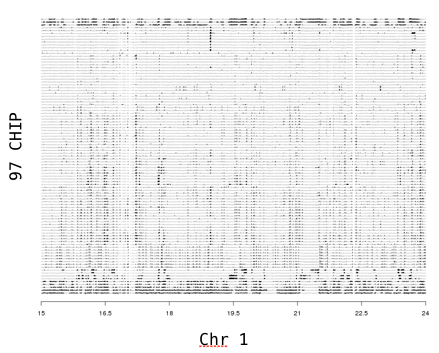
\includegraphics[width=0.5\columnwidth]{mat}
              \caption{CHIPseq Profiles in H1-hESC (Human embryonic stem cell). These profiles [2] were used in constructing color classification.}
      	\end{figure}       
      \end{block}

     
      %-- Block 1-4
      \begin{block}{Chromatin States of hESC}
  		\begin{figure}
   			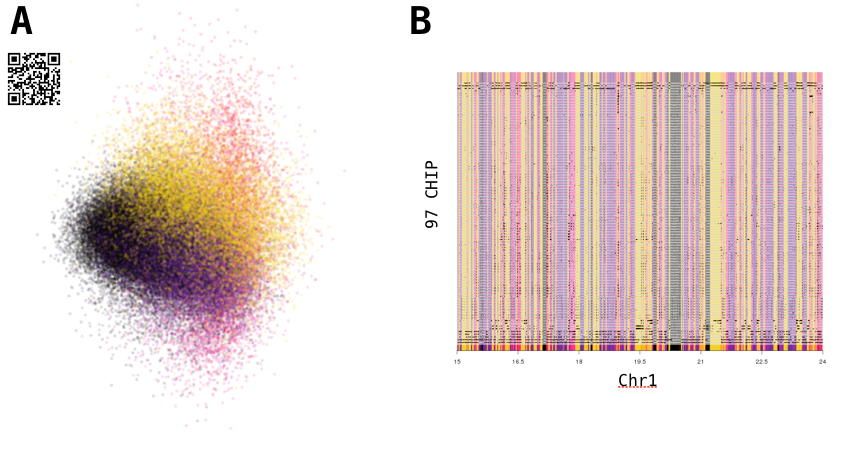
\includegraphics[width=.9\textwidth]{clusteredAnimatedPC}
			\caption{A) 3D PCA projection. Colors representing distinct chromatin states. Barcode encodes the URL (https://dl.dropbox.com/u/82788830/human-1PC.mov) to play 3D PCA. B) Representation of Color States across CHIPseq profiles in a detail of chromosome 1. Five clusters were built as color states consisting of black, purple, yellow, pink, and red.}
  		\end{figure}
	  \end{block}
    \end{column}
  
       
    %-- Column 2 ---------------------------------------------------
    \begin{column}{0.32\linewidth}

      %-- Block 2-1
      \begin{block}{Chromosome Painting}
        \begin{figure}
   			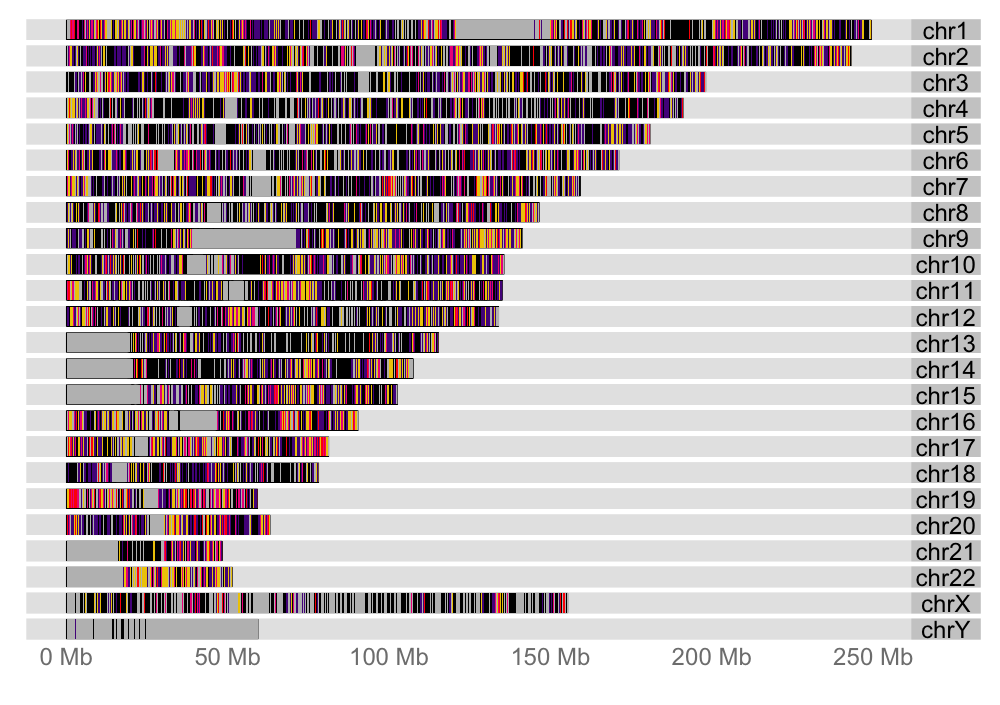
\includegraphics[width=1\textwidth]{chromatinpainted}
			\caption{Color States Painted across all Chromosomes. Gray zones indicate regions of repeats.}
  		\end{figure}
      
	  \end{block}
      %-- Block 2-2
      \begin{block}{Ingredients}
      
		\begin{figure}
			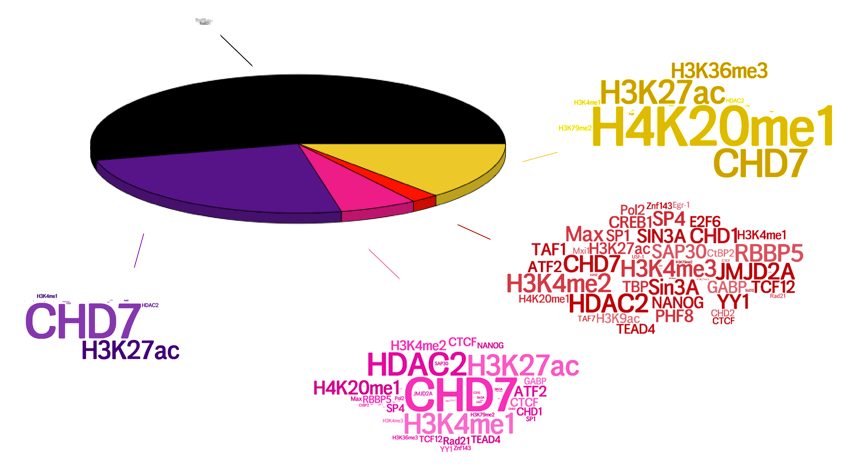
\includegraphics[width=1\textwidth]{H1pizza}
			\caption{Chromatin Marks Enriched in Color. The word's size reflects the degree of enrichment. The percentage represents the coverage of each color in our genome.}
		\end{figure}
		
      \end{block}
            
       %-- Block 2-3
      \begin{block}{Genomic Features}
      		\begin{figure}
					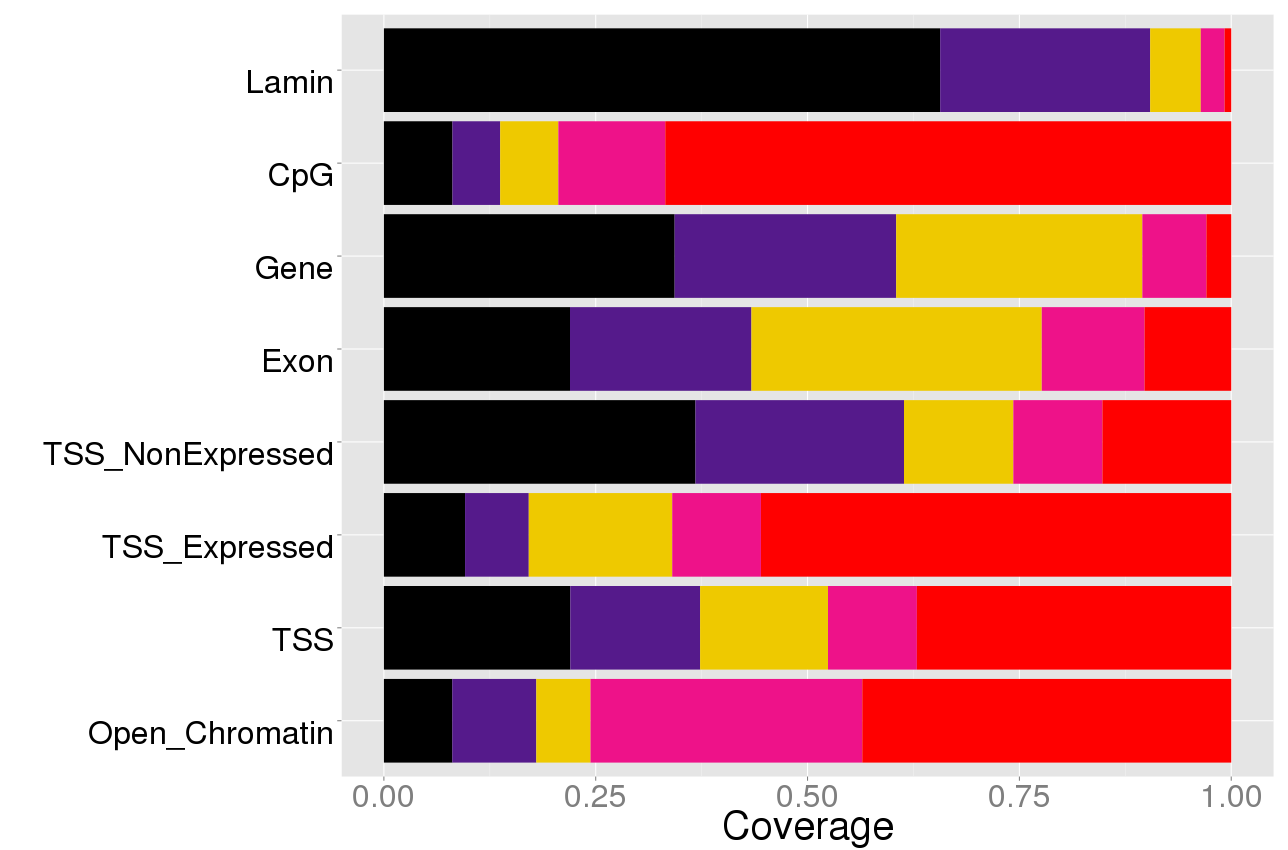
\includegraphics[width=1\textwidth]{GenomicFeatures}
					\caption{Genomic Features over Color Chromatin. The width of the bar indicates the proportion of the given feature that lies in the chromatin type. TSS: transcription start site}
			\end{figure}
      \end{block}



    \end{column}%2

    %-- Column 3 ---------------------------------------------------
    \begin{column}{0.32\linewidth}

      %-- Block 3-1
      \begin{block}{Our Answer: Take-Home Message}
       
       \lettrine[lines=1,findent=0pt, nindent=1pt]{!`YES!}{ We Have Black in Our Chromatin.}\\[20pt]
        
        \lettrine[lines=1,findent=0pt, nindent=1pt]{C}{haracteristics} of our black chromatin:
        \begin{itemize}
        	  \item Wide-spread, sheltering about half of our genome
          \item Uncharted epigenetics markers, hardly no enrichment of the known histone marks or transcription factors
          \item Rich in LADs (Lamina-associated Domains) but CpG-poor
          \item Genic regions, covering about 35\% of our genes
          \item Repressive genic regions, genes in black are not expressed, or expressed at low level
          \item Low proportion of open-chromatin\\[20pt]
        \end{itemize} 
        
       \begin{shadequote}
      	The thing that doesn't fit is the most interesting -Richard Feynman 	
      \end{shadequote}
        
      \end{block}
      
      %-- Block 3-2
      \begin{block}{?`Can we Trust Encode?}
   
      \lettrine[lines=1,findent=0pt, nindent=1pt]{C}{hallenges} in the H1-hESC's CHIPseq dataset (downloaded in 2012) include:\\[10pt]
      
      \begin{itemize}
      	\item Genome release artifact. Lift-over from hg18 to hg19 clusters profiles based on the original release they were mapped. The profiles had to be mapped again using the raw data. \\[30pt]
			\begin{figure}
					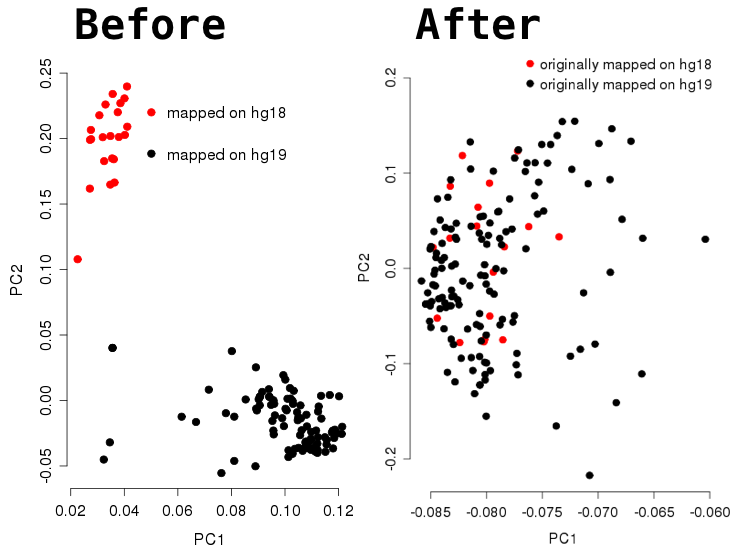
\includegraphics[width=.8\textwidth]{liftover}
					\caption{PCA of CHIPseq Profiles. Before (lift-over hg18-hg19): profiles cluster based on the release they were mapped. After (remapping FASTQ files, profiles no longer cluster based on the release)}
					
					
			\end{figure}
		\item The integrity of three CHIPseq profiles could not be confirmed, as they failed the md5sum check verification.
		\item Out of 158 CHIPseq profiles, 65 profiles do not pass the FASTQC tests.
      
    
      \end{itemize}
      
      \end{block}

      %-- Block 3-3
      \begin{block}{References \& Acknowledgment}
      	\begin{enumerate}
      		\item Filion, G. J. et al. Systematic Protein Location Mapping Reveals Five Principal Chromatin Types in Drosophila Cells. Cell, 2010.
      		\item ENCODE Project Consortium, et al. A user's guide to the encyclopedia of DNA elements (ENCODE). PLoS Biol, 2011.\\[45pt]
		\end{enumerate}
		

	   \begin{shadequote}
      	Special thanks to you for reading our poster. We do hope you enjoy reading it. If you feel like giving some comments, questions, or (thoughtful) gifts maybe :) , please feel free to contact us.	
      \end{shadequote}
		
      \end{block}

    \end{column}%3

  \end{columns}
\end{frame}
\end{document}